
iTaken from \fullcite{gery19book}

%.........................................
\paragraph{Rotation of elastic stresses}.

\begin{multicols}{2}
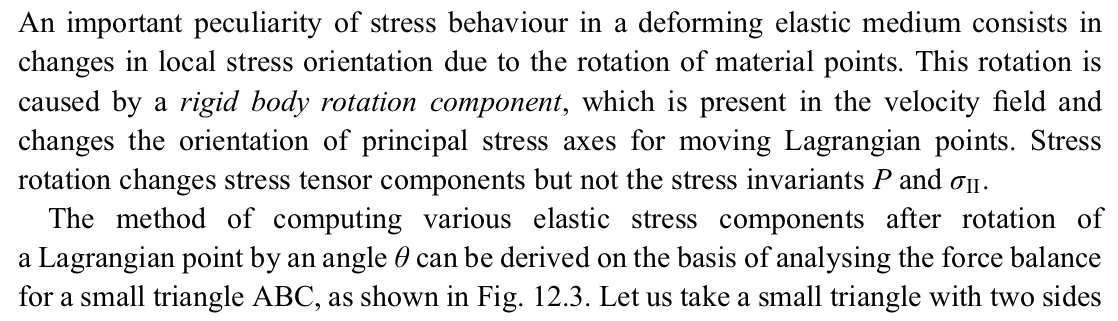
\includegraphics[width=8.3cm]{images/viscoelasticity/geryabook_1}
\end{multicols}

\begin{multicols}{2}
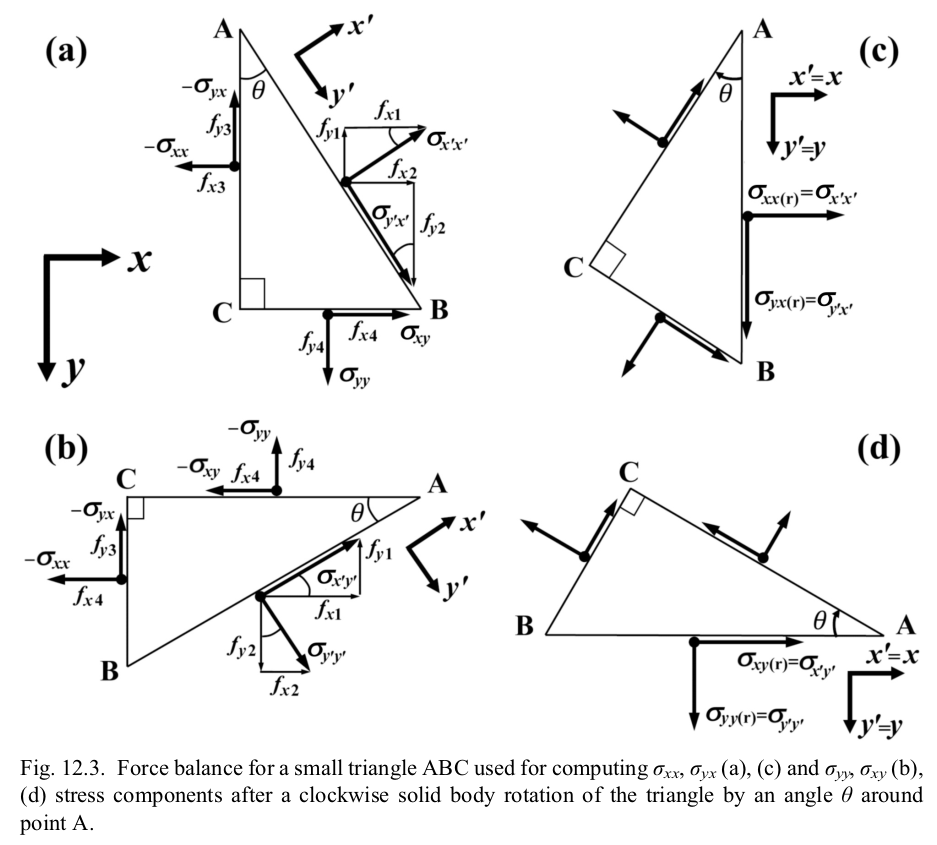
\includegraphics[width=8.3cm]{images/viscoelasticity/geryabook_19}
\end{multicols}

\begin{multicols}{2}
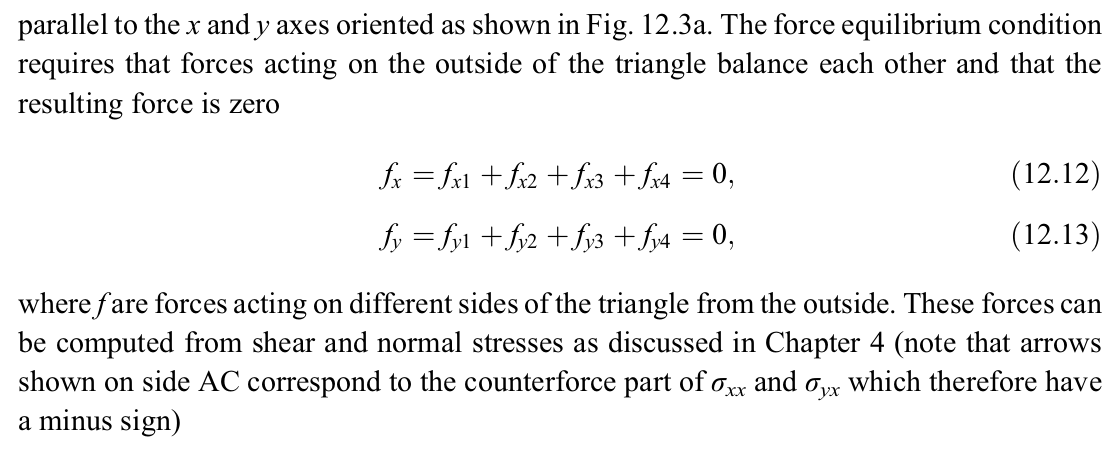
\includegraphics[width=8.3cm]{images/viscoelasticity/geryabook_2}
\end{multicols}

\begin{multicols}{2}
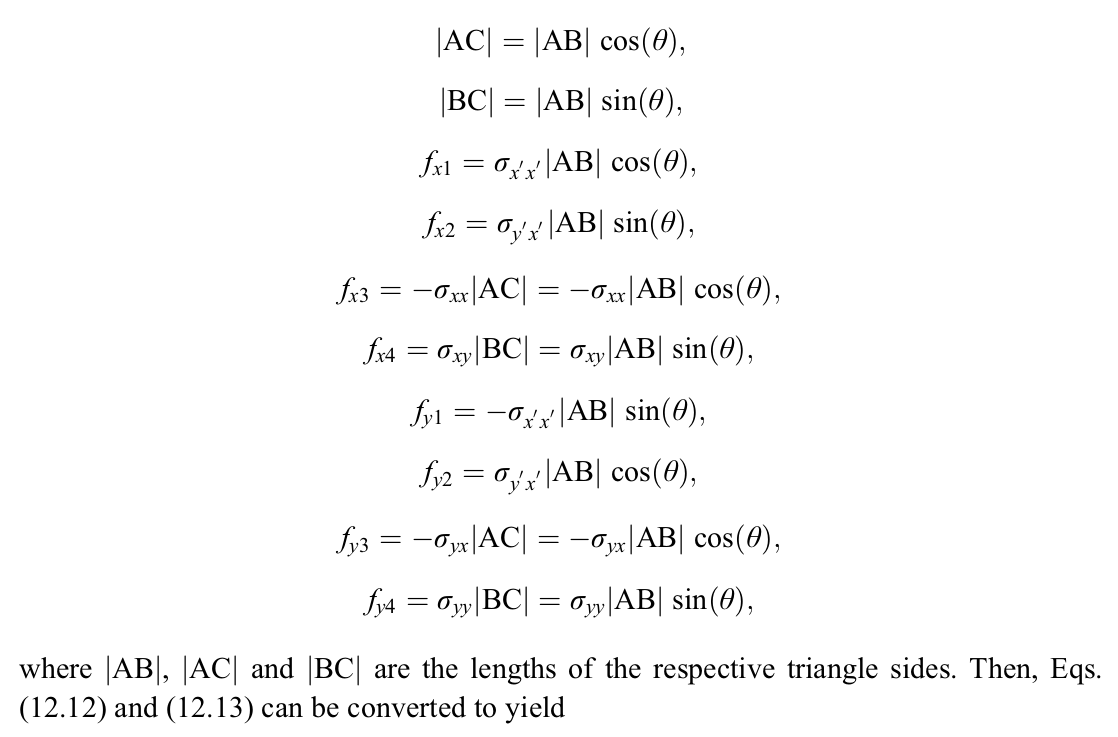
\includegraphics[width=8.3cm]{images/viscoelasticity/geryabook_3}
\end{multicols}

\begin{multicols}{2}
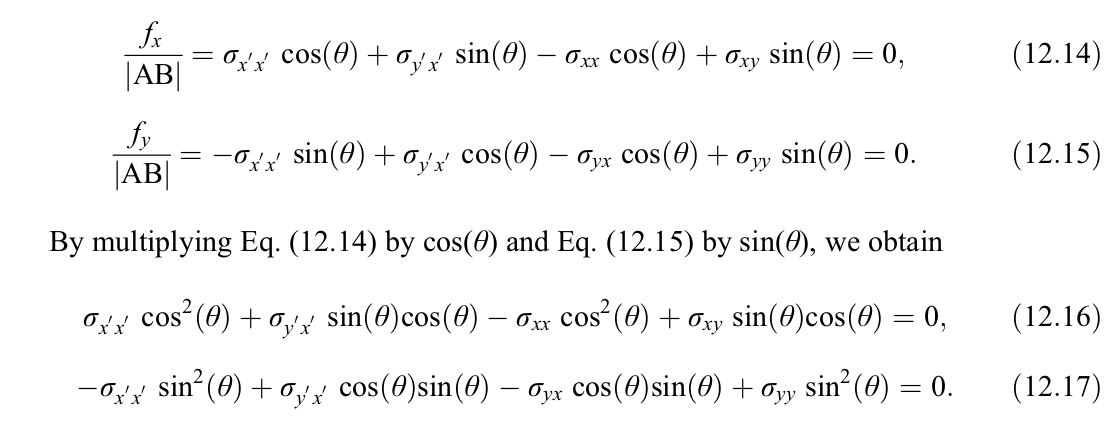
\includegraphics[width=8.3cm]{images/viscoelasticity/geryabook_4}
\end{multicols}

\begin{multicols}{2}
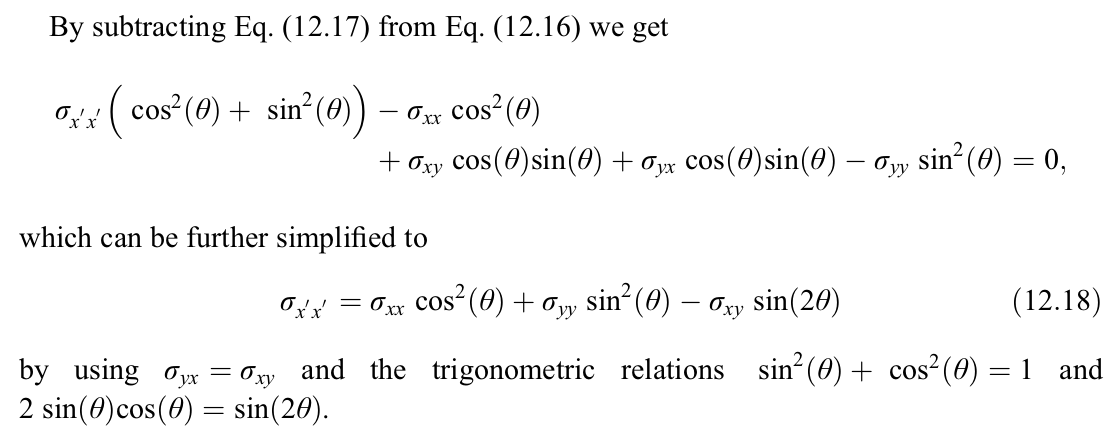
\includegraphics[width=8.3cm]{images/viscoelasticity/geryabook_5}
\end{multicols}

\begin{multicols}{2}
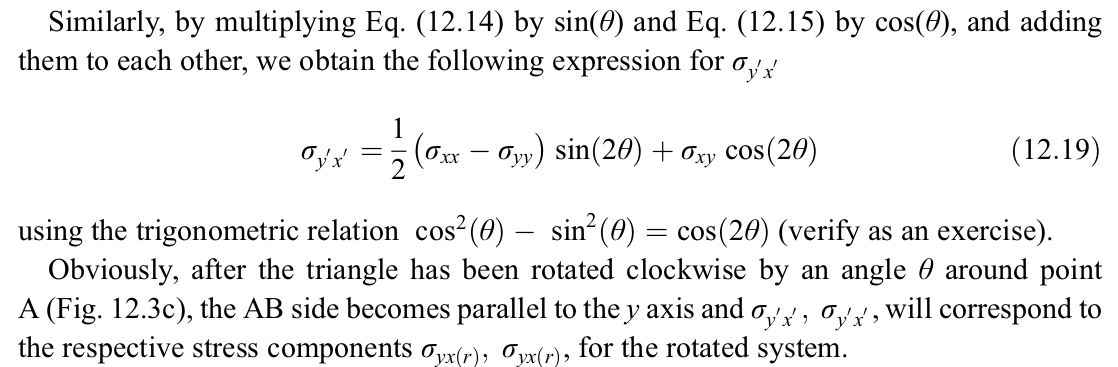
\includegraphics[width=8.3cm]{images/viscoelasticity/geryabook_6}
\end{multicols}

\begin{multicols}{2}
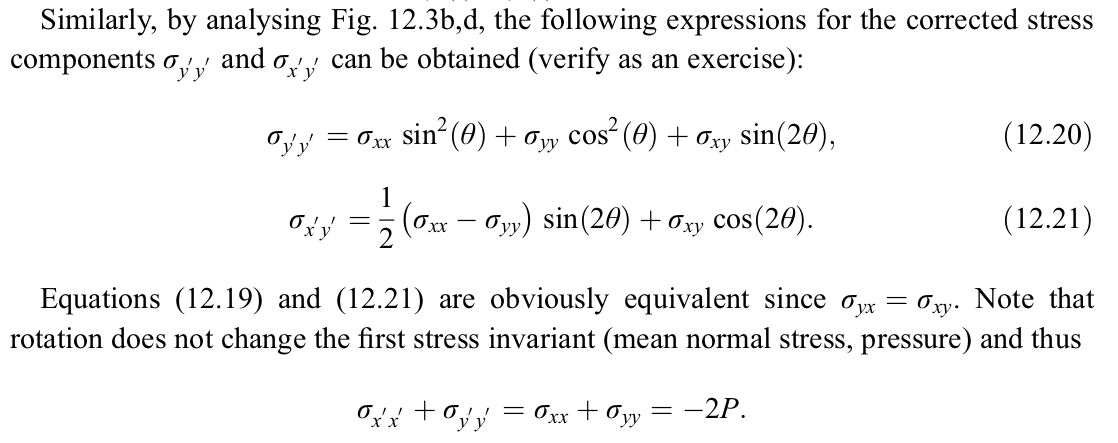
\includegraphics[width=8.3cm]{images/viscoelasticity/geryabook_7}
\end{multicols}

\begin{multicols}{2}
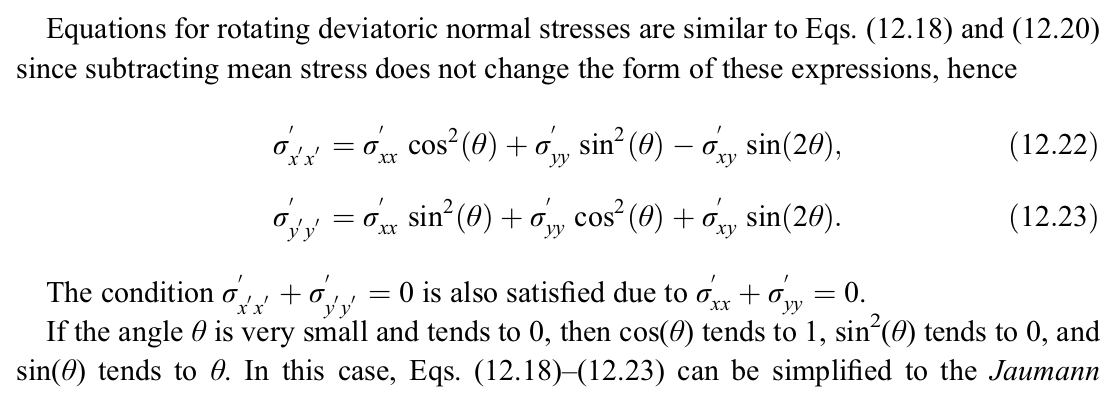
\includegraphics[width=8.3cm]{images/viscoelasticity/geryabook_8}
\end{multicols}

\begin{multicols}{2}
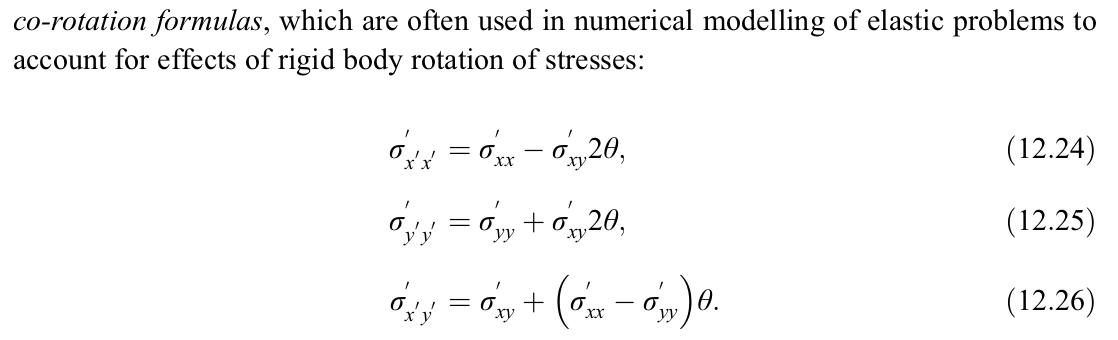
\includegraphics[width=8.3cm]{images/viscoelasticity/geryabook_9}
\end{multicols}

\begin{multicols}{2}
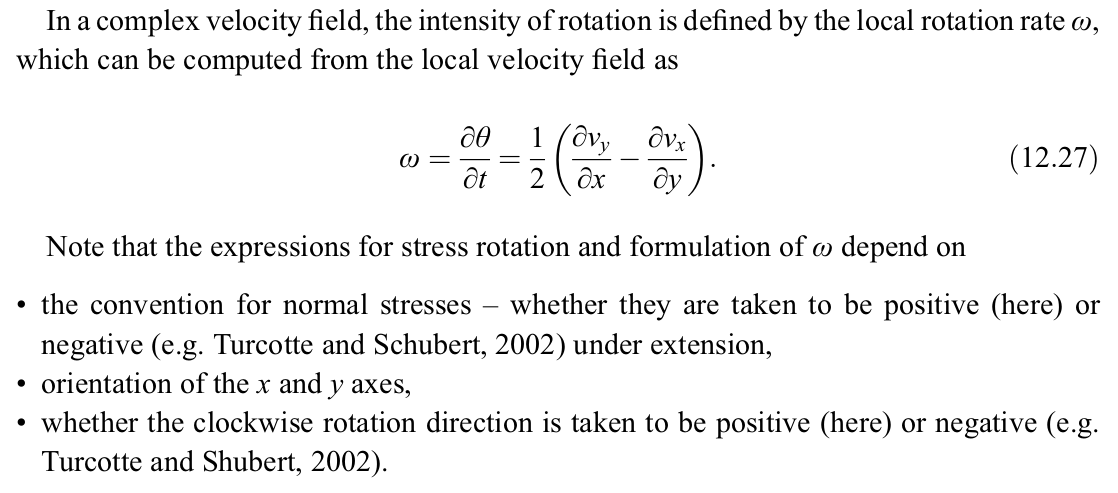
\includegraphics[width=8.3cm]{images/viscoelasticity/geryabook_10}
\end{multicols}

\begin{multicols}{2}
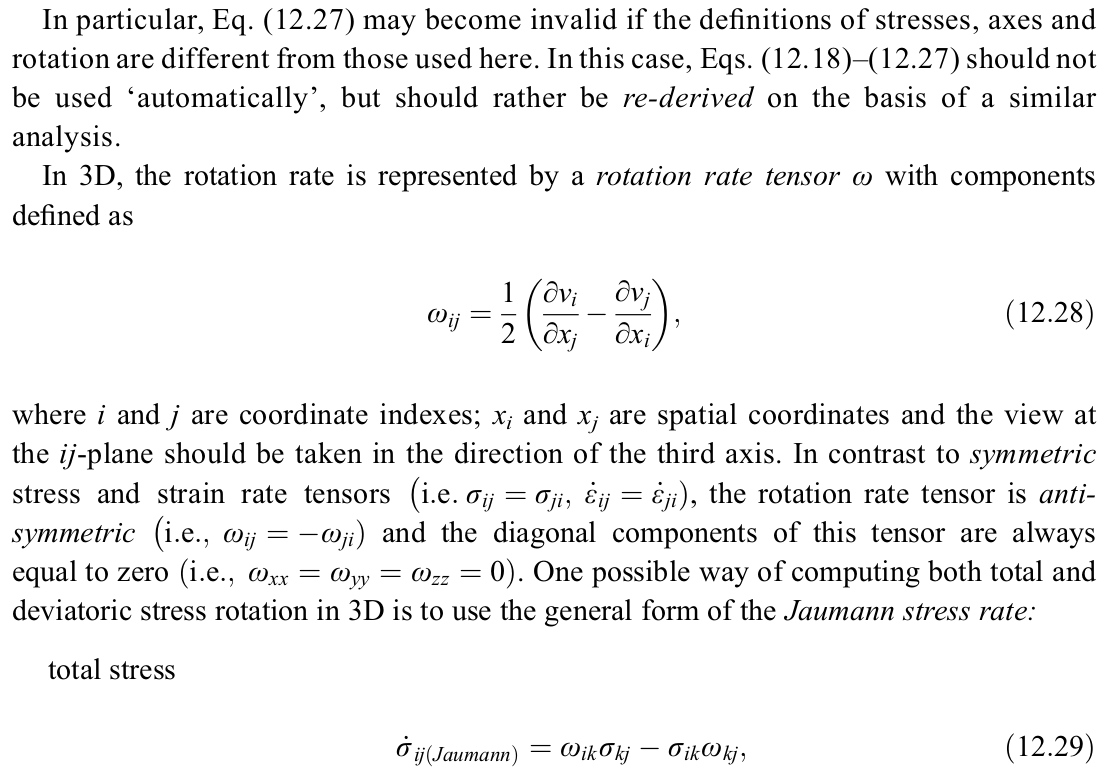
\includegraphics[width=8.3cm]{images/viscoelasticity/geryabook_11}
\end{multicols}

\begin{multicols}{2}
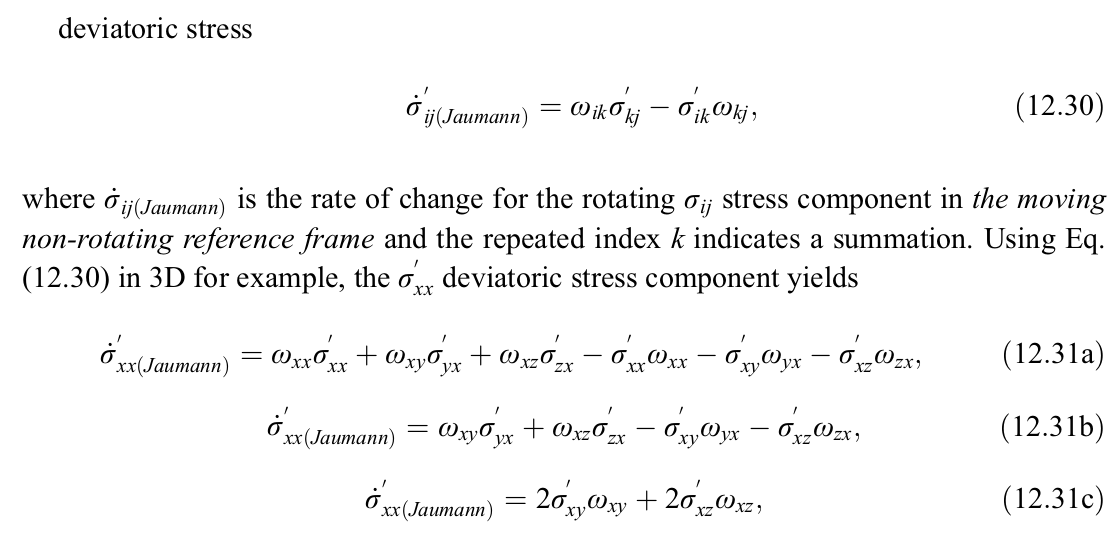
\includegraphics[width=8.3cm]{images/viscoelasticity/geryabook_12}
\end{multicols}

\begin{multicols}{2}
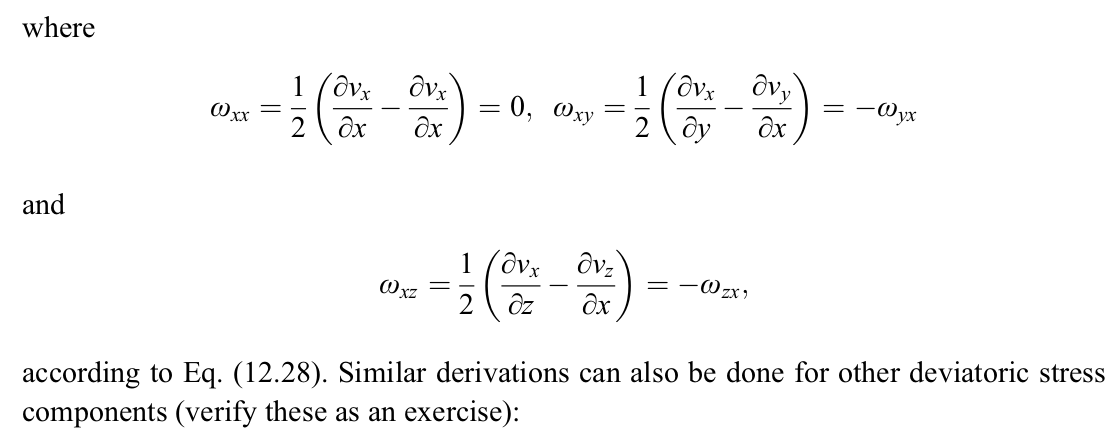
\includegraphics[width=8.3cm]{images/viscoelasticity/geryabook_13}
\end{multicols}

\begin{multicols}{2}
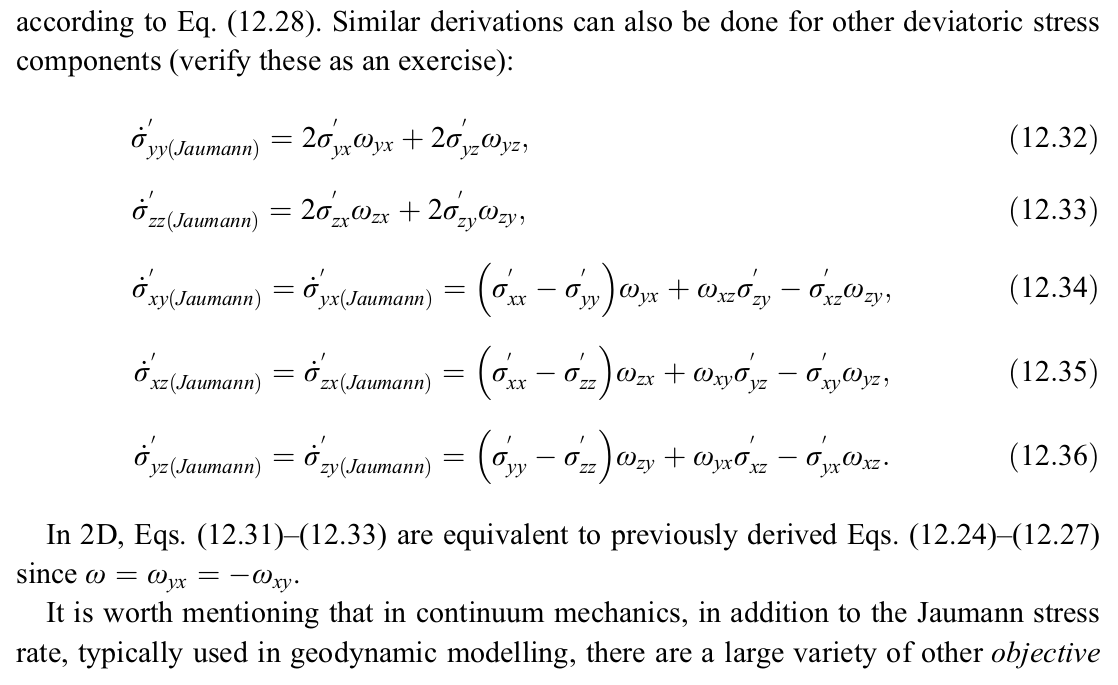
\includegraphics[width=8.3cm]{images/viscoelasticity/geryabook_14}
\end{multicols}

\begin{multicols}{2}
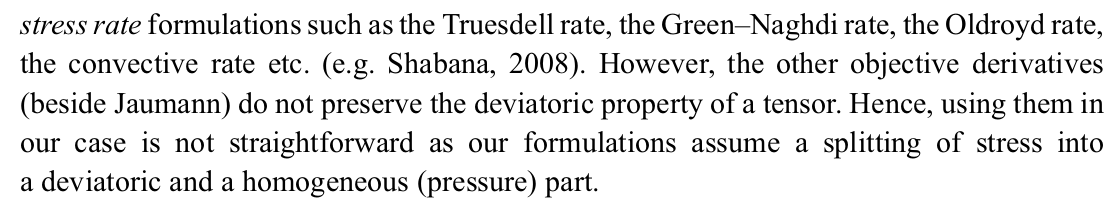
\includegraphics[width=8.3cm]{images/viscoelasticity/geryabook_15}
\end{multicols}

\begin{multicols}{2}
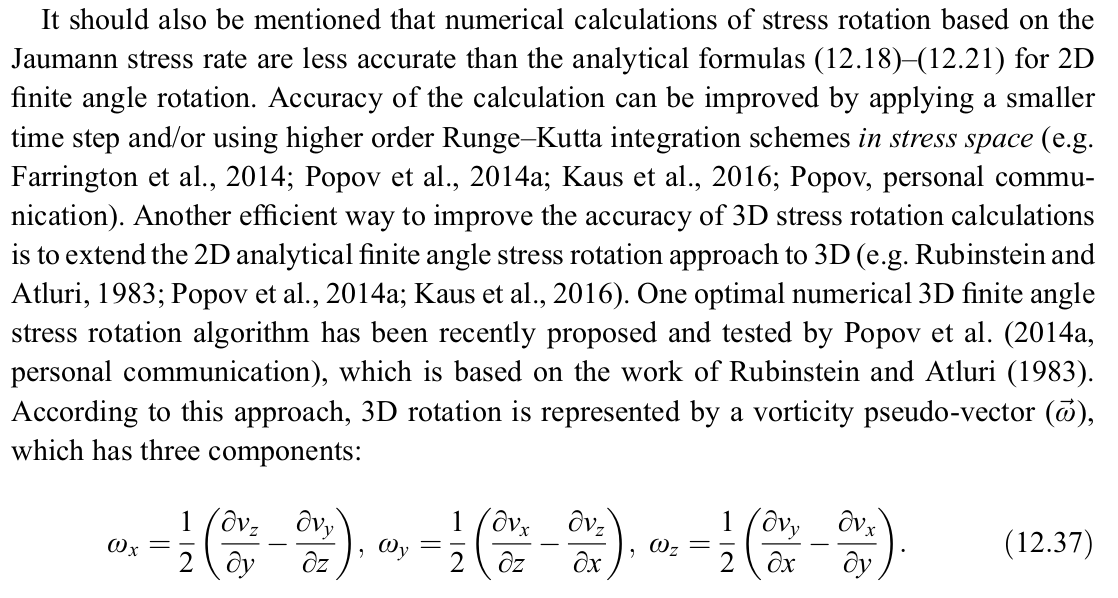
\includegraphics[width=8.3cm]{images/viscoelasticity/geryabook_16} 
\end{multicols}

\begin{multicols}{2}
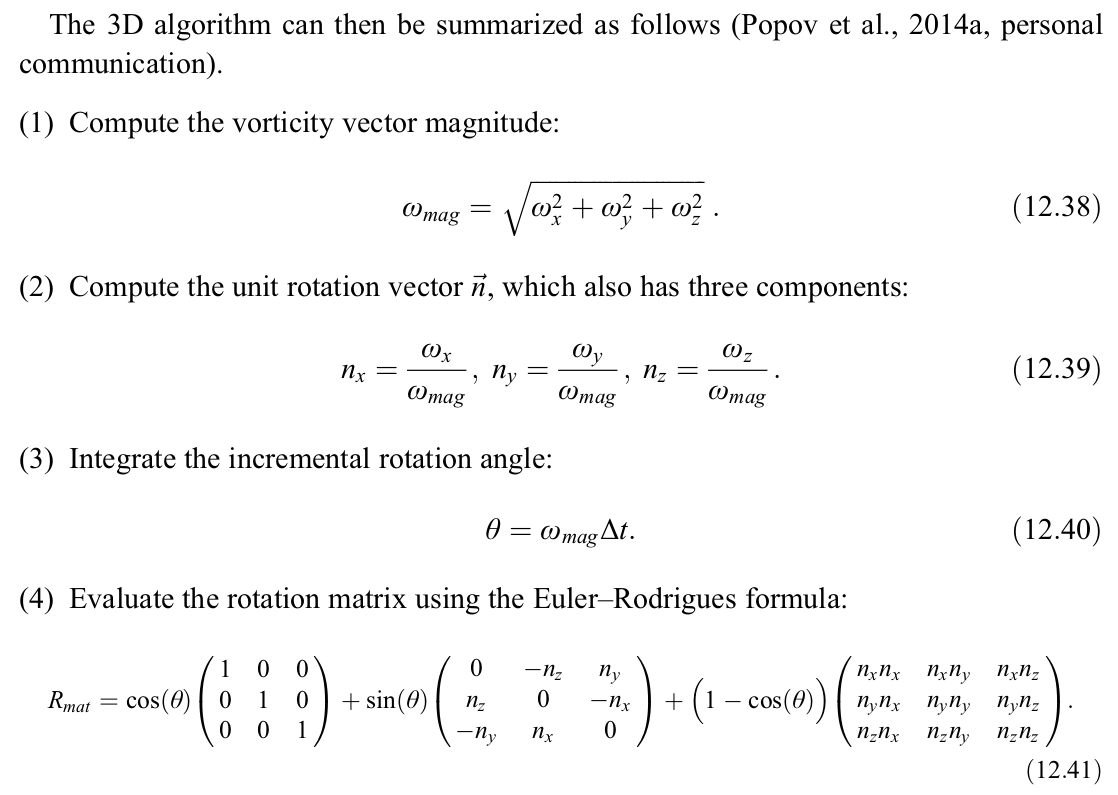
\includegraphics[width=8.3cm]{images/viscoelasticity/geryabook_17}
\end{multicols}

\begin{multicols}{2}
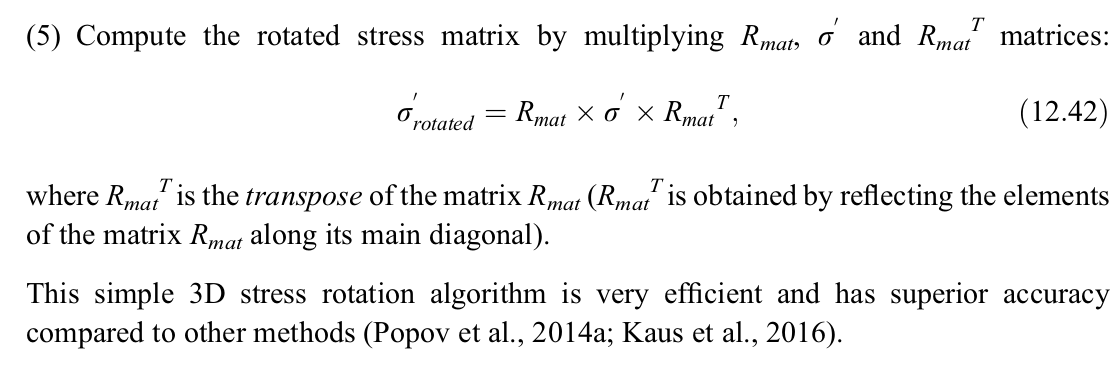
\includegraphics[width=8.3cm]{images/viscoelasticity/geryabook_18}
\end{multicols}

%.........................................
\paragraph{Maxwell visco-elastic rheology}.

Despite different notations we find that the book follows the standard approach.

\begin{multicols}{2}
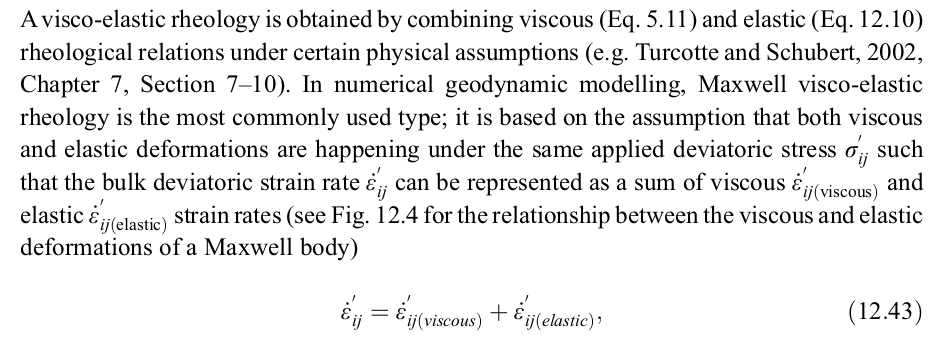
\includegraphics[width=8.3cm]{images/viscoelasticity/geryabook_20} \\
\[
\dot{\bm\varepsilon}_{\rm T}^d = 
\dot{\bm\varepsilon}_{\rm v}^d + 
\dot{\bm\varepsilon}_{\rm e}^d
\]

\end{multicols}

\begin{multicols}{2}
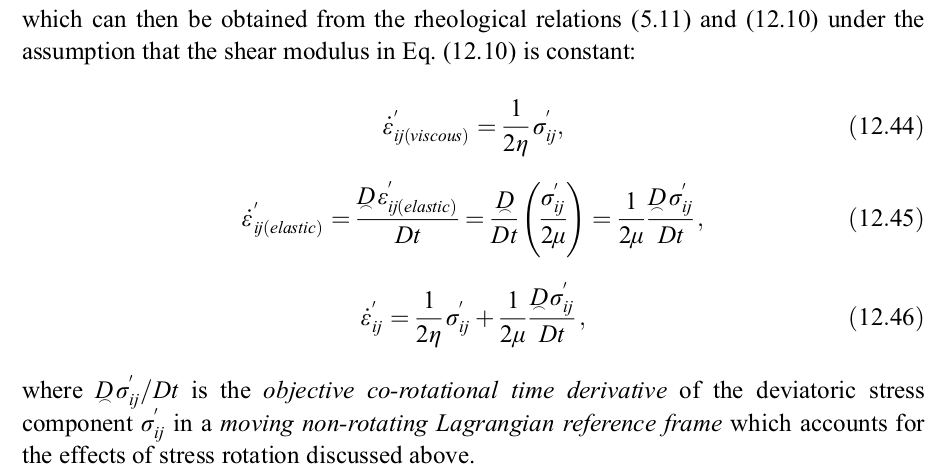
\includegraphics[width=8.3cm]{images/viscoelasticity/geryabook_21} \\
\[
\dot{\bm\varepsilon}_{\rm T}^d  = \frac{1}{2\eta} {\bm \tau} + \frac{1}{2\mu} \check{\bm \tau}
\]
where $\check{\bm \tau}$ is the objective co-rotational  time derivative of the deviatoric stress.

\end{multicols}

\begin{multicols}{2}
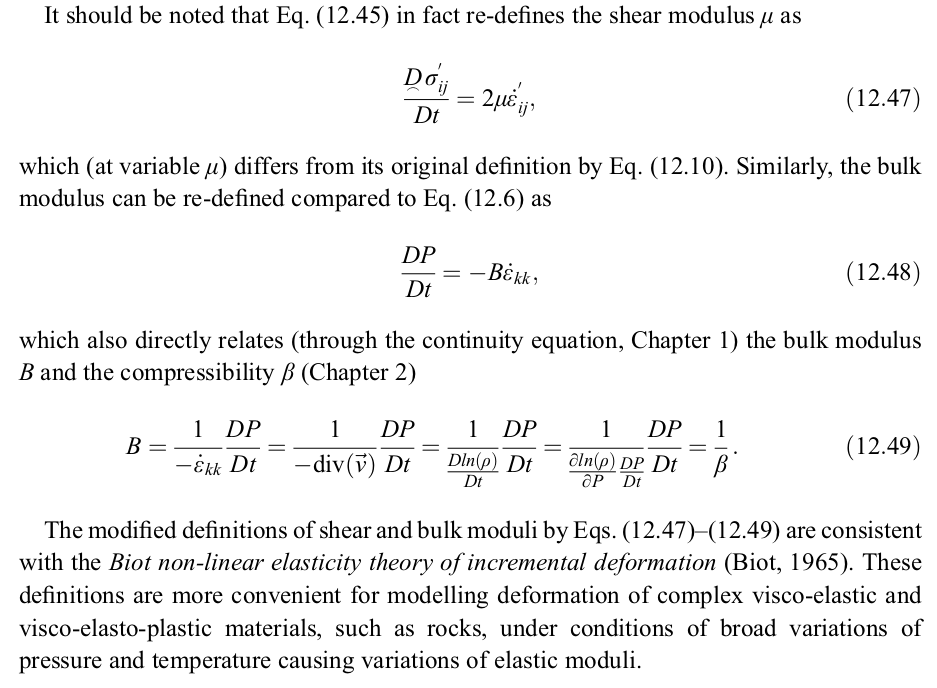
\includegraphics[width=8.3cm]{images/viscoelasticity/geryabook_22}
\end{multicols}



